\documentclass[10pt, a4paper]{article}

%%% SST LAB PROTOCOLL PREAMBLE
%%% 2019
%%%%%%%%%%%%%%%%%%%%%%%%%%%%%%%


%%% PACKAGES
%%%%%%%%%%%%%%%%%%%%%%%%%%%

\usepackage[ngerman]{babel}

\usepackage[utf8]{inputenc}
\usepackage{amsmath}
\usepackage{pgfplots}
\usepackage{tikz}
\usepackage[many]{tcolorbox}
\usepackage{graphicx}
\graphicspath{ {./graphics/} }
\usepackage{pdfpages}
\usepackage{dashrule}
\usepackage{float}
\usepackage{siunitx}
\usepackage{trfsigns}
\usepackage{booktabs}
\usepackage[european]{circuitikz}
\usepackage{tcolorbox}

%%% DOCUMENT GEOMETRY
%%%%%%%%%%%%%%%%%%%%%%%%%%%

\usepackage{geometry}
\geometry{
 a4paper,
 total={0.6180339887498948\paperwidth,0.6180339887498948\paperheight},
 top = 0.1458980337503154\paperheight,
 bottom = 0.1458980337503154\paperheight
 }
\setlength{\jot}{0.013155617496424828\paperheight}
\linespread{1.1458980337503154}

\setlength{\parskip}{0.013155617496424828\paperheight} % paragraph spacing


%%% COLORS
%%%%%%%%%%%%%%%%%%%%%%%%%%%

\definecolor{red1}{HTML}{f38181}
\definecolor{yellow1}{HTML}{fce38a}
\definecolor{green1}{HTML}{95e1d3}
\definecolor{blue1}{HTML}{66bfbf}
\definecolor{hsblue}{HTML}{00b1db}
\definecolor{hsgrey}{HTML}{afafaf}

%%% CONSTANTS
%%%%%%%%%%%%%%%%%%%%%%%%%%%
\newlength{\smallvert}
\setlength{\smallvert}{0.0131556\paperheight}


%%% COMMANDS
%%%%%%%%%%%%%%%%%%%%%%%%%%%

% differential d
\newcommand*\dif{\mathop{}\!\mathrm{d}}

% horizontal line
\newcommand{\holine}[1]{
  	\begin{center}
	  	\noindent{\color{hsgrey}\hdashrule[0ex]{#1}{1pt}{3mm}}\\%[0.0131556\paperheight]
  	\end{center}
}

% mini section
\newcommand{\minisec}[1]{ \noindent\underline{\textit {#1} } \\}

% quick function plot
\newcommand{\plotfun}[3]{
  \vspace{0.021286\paperheight}
  \begin{center}
    \begin{tikzpicture}
      \begin{axis}[
        axis x line=center,
        axis y line=center,
        ]
        \addplot[draw=red1][domain=#2:#3]{#1};
      \end{axis}
    \end{tikzpicture}
  \end{center}
}

% box for notes
\newcommand{\notebox}[1]{

\tcbset{colback=white,colframe=green1!100!black,title=Note!,width=0.618\paperwidth,arc=0pt}

 \begin{center}
  \begin{tcolorbox}[]
   #1 
  \end{tcolorbox}
 
 \end{center} 
 
}

% box for equation
\newcommand{\eqbox}[2]{
	
	\tcbset{colback=white,colframe=green1!100!black,title=,width=#2,arc=0pt}
	
	\begin{center}
		\begin{tcolorbox}[ams align*]
				#1
		\end{tcolorbox}
		
	\end{center} 
	
}
% END OF PREAMBLE

%\addbibresource{sources.bib}
%\addbibresource{web.bib}

\begin{document}

%
\includepdf{./titlepage/titlepage.pdf}
%\pagebreak

\begin{center}
  \Large{Einfacher Masse-Feder-Dämpfer Performancebenchmark in Rust}
\end{center}

\begin{flushright}
  R. Grünert\\
  \today
\end{flushright}

\begin{flushleft}
  CPU: i7 4790k
\end{flushleft}

\section{Umsetzung}
In diesem Projekt wurde die Eulermethode zur numerischen Lösung der Differentialgleichung eines einfachen Mass-Feder-Dämpfer-Modells genutzt, um den Speedup bei der parallelen Verarbeitung zu untersuchen. Dabei werden mehrere Lösungen der Trajektorien für zufällige Dämpfungsfaktoren ermittelt und gemittelt. Die Lösungsaufgaben werden im Fall der Parallelverarbeitung gleichmäßig auf die Verarbeitungseinheiten aufgeteilt und anschließend ebenfalls gemittelt.\\

Rust stellt für den Multicore-Betrieb die crate \inlinecodee{std::thread} zur Verfügung. Diese bietet die Funktion \inlinecodee{spawn} zur Erstellung eines neuen Threads auf Basis der gegebenen Funktion. Man erhält einen \inlinecodee{JoinHandle} für diesen Thread. Mittels \inlinecodee{join}-Methode kann dann auf die Terminierung des Threads gewartet und das Ergebnis \glqq{}eingesammelt\grqq{} werden. Es folgt ein Beispiel:

\begin{minted}{rust}
  let handle: std::thread::JoinHandle<f32> = std::thread::spawn(|| {
    1.0 + 1.0
  });

  result = handle.join()?; // 2.0
\end{minted}
\medskip

Spawnt man mehrere Threads, werden diese bereits automatisch auf die CPU-Verarbeitungseinheiten aufgeteilt. Um Kernaffinitäten zu spezifizieren, bietet sich die \inlinecodee{core\_affinity} crate an, welche sich einfach in die Threadfunktion integriert.

\section{Ausführung}
Die sequentielle und parallele Lösung wurden jeweils mit dem Optiomierungslevel \inlinecodee{release} kompiliert. Beide erhielten dann eine Gesamtzahl von 2000000 Lösungen.\\

Zur Ausführung des parallelen Programmes kann der Befehl \inlinecodee{cargo run --release -- 20000000 run-stepped} verwendet werden. Dabei sind folgene Aufrufargumente notwendig:

\begin{minted}{text}
Usage: MassSpringDamper_Euler_Benchmark <NUM_RUNS> <COMMAND>

Commands:
  run-cores    Run on specific cores
  run-all      Run on all available cores
  run-stepped  Run on all cores, increasing the core count each time
  help         Print this message or the help of the given subcommand(s)

Arguments:
  <NUM_RUNS>  Total number of computations

Options:
  -h, --help     Print help
  -V, --version  Print version
\end{minted}

\section{Ergebnisse}

Das Script \inlinecodee{plot.R} erstellt einen Graphen der zuletzt berechneten Trajeketorie des Systems , ein Beispiel ist in Abb. \ref{fig:trajectory} zu sehen.
Mit dem Script \inlinecodee{plot\_amdahl.R} kann der speedup aus der Datei \inlinecodee{speeds.csv} grafisch dargestellt werden. Dabei werden die Dateien \inlinecodee{plot\_amdahl\_duration.pdf} und \inlinecodee{plot\_amdahl\_speedup.pdf} erstellt. Abb. \ref{fig:speedop} zeigt das Ergebnis. Der Speedup läuft bis zu 4 Kernen fast perfekt linear, ab 5 Kernen gibt es allerdings einen negativen Sprung, welcher Möglicherweise auf Hyperthreading zurückzuführen ist.

\begin{figure}[h]
  \begin{center}
    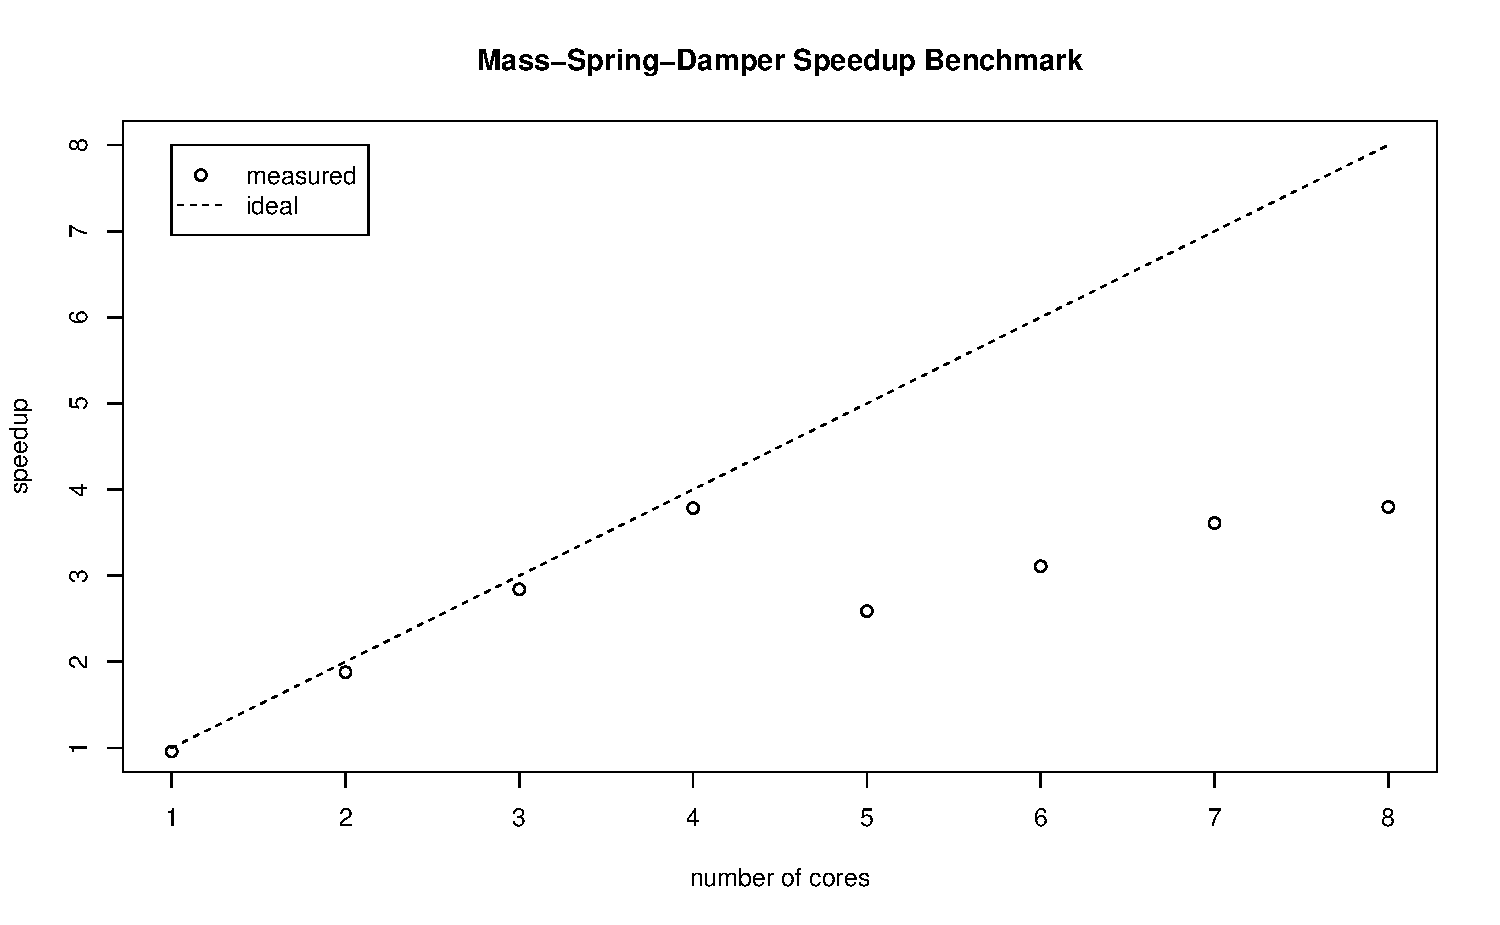
\includegraphics[width=\textwidth]{graphics/plot_amdahl_speedup_2M.pdf}
  \end{center}
  \caption{Benchmarkergebnis zum Speedup.}\label{fig:speedop}
\end{figure}


\begin{figure}[h]
  \begin{center}
    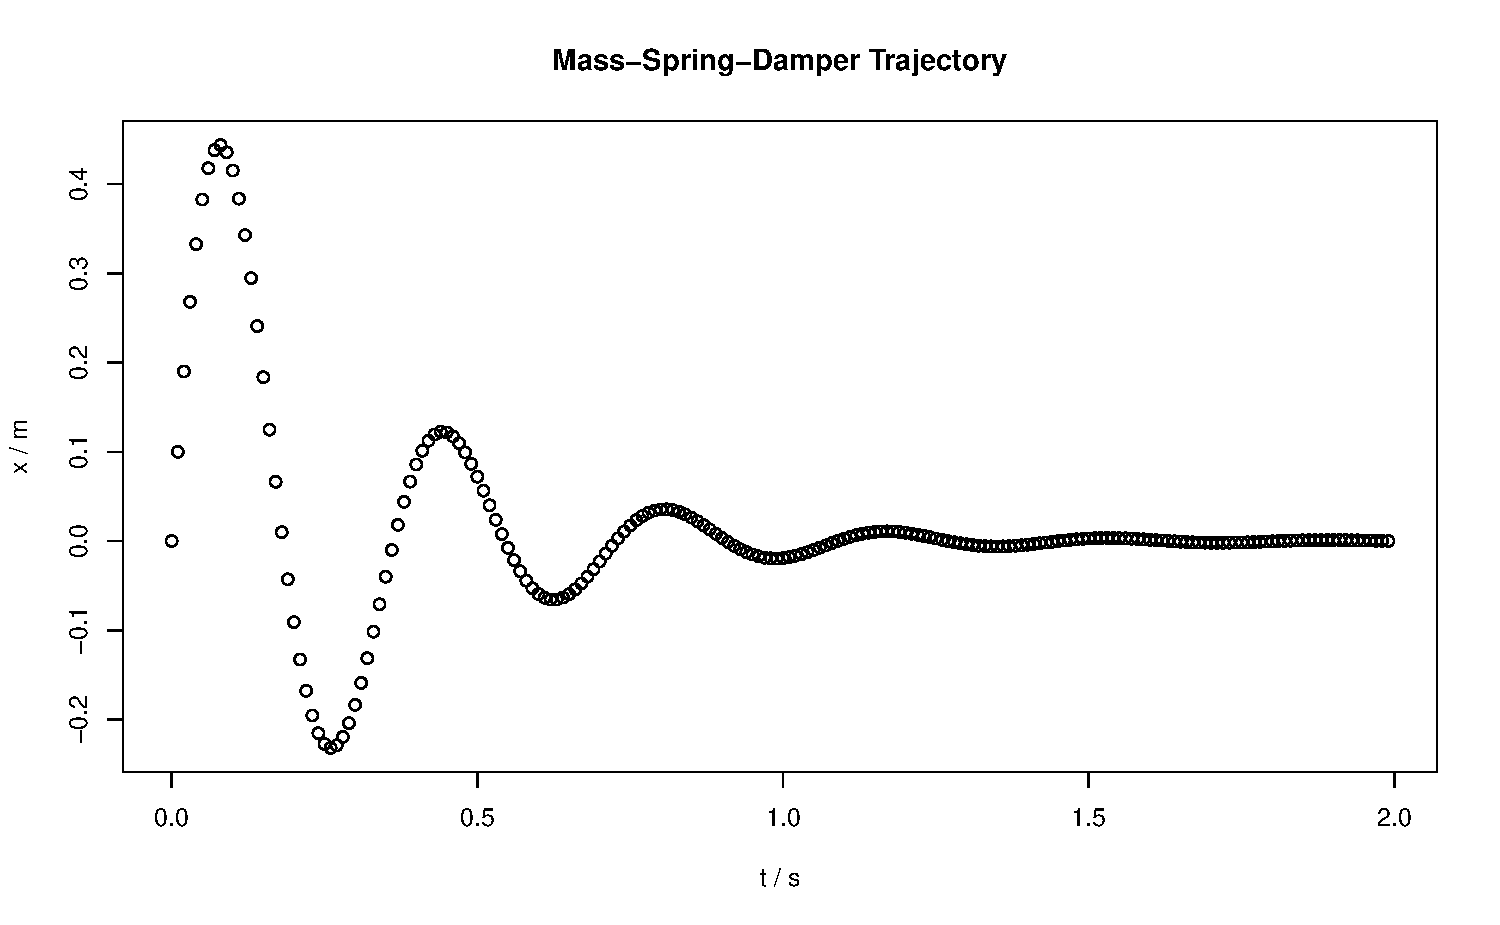
\includegraphics[width=\textwidth]{graphics/trajectory.pdf}
  \end{center}
  \caption{Beispieltrajektorie.}\label{fig:trajectory}
\end{figure}




\section{Mögliche Verbesserungen}
\begin{itemize}
  \item Die Funktion \inlinecodee{MSDThreads::spawn\_threads} sollte eigentlich eine Closure als Aufrufparameter erhalten, welche die Basis-\inlinecodee{MSDParameter} bindet und die Funktion somit unabhängig von der eigentlichen MFD-Problemstellung macht
  \item Das Teilen der Basisparameter des MFD-Systems könnte einfacher über \inlinecodee{Arc}-Typen geschehen, statt eine statische Lebensdauer zu fordern
  \item Warnungen beseitigen
  \item Test auf anderer CPU, möglicherweise mit mehr Kernen
\end{itemize}

% ------------------------------------------------------------------------------

%\printbibheading
%\begin{refsection}[sources.bib]
%\nocite{*}
%\printbibliography[heading=subbibliography,title={Literature}]
%\end{refsection}

%\begin{refsection}[web.bib]
%\nocite{*}
%\printbibliography[heading=subbibliography,title={Web}]
%\end{refsection}

%\begin{refsection}[software.bib]
%\nocite{*}
%\printbibliography[heading=subbibliography,title={Software Used}]
%\end{refsection}


%\begin{figure}[H]
    \centering
    \begin{minipage}{0.48\textwidth}
        \centering
        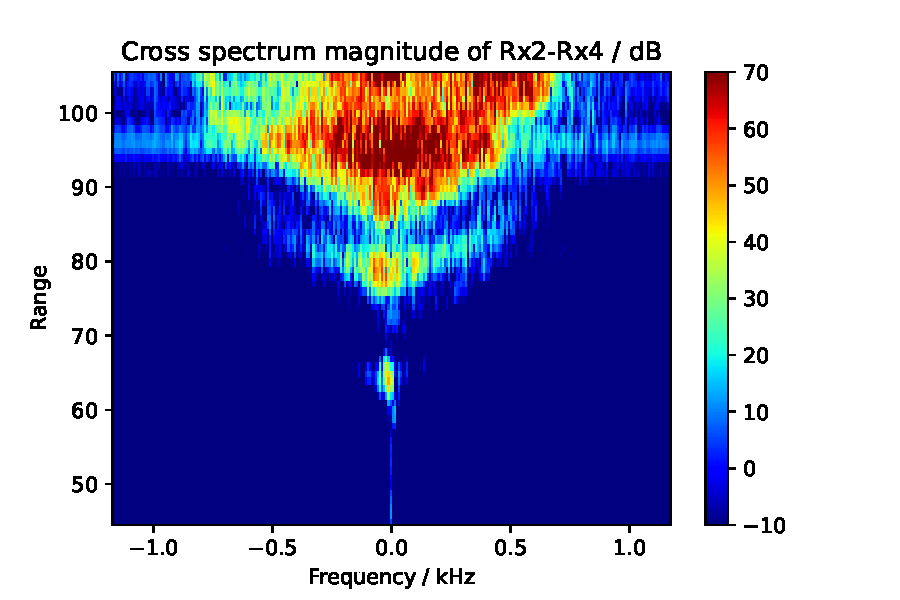
\includegraphics[width=\textwidth]{graphics/t4/t4-mag-2-4.pdf}
    \caption{Task 4: Magnitude of cross spectrum of Receivers 2 and 4.}
    \label{fig:t4-mag-2-4}
    \end{minipage}\hfill
    \begin{minipage}{0.48\textwidth}
        \centering
             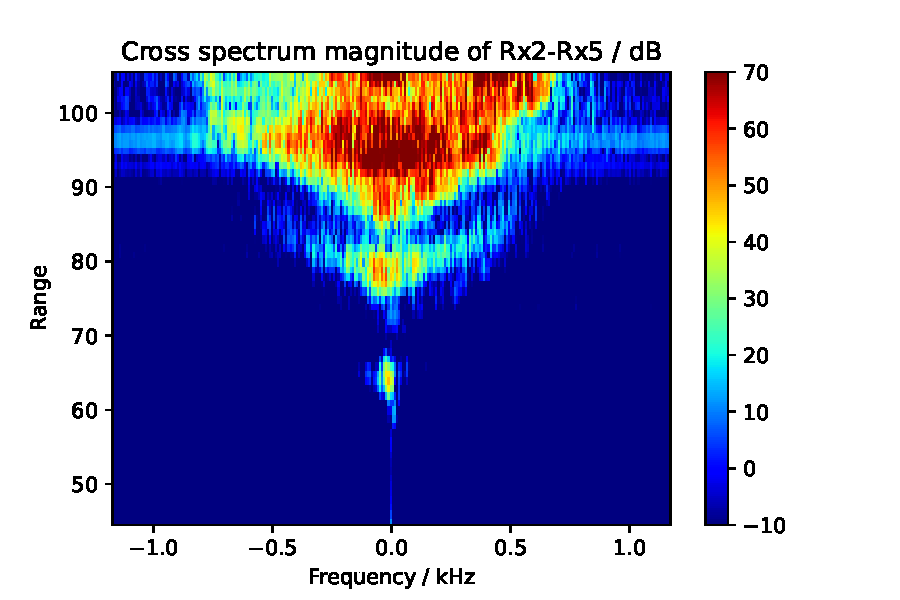
\includegraphics[width=\textwidth]{graphics/t4/t4-mag-2-5.pdf}
    \caption{Task 4: Magnitude of cross spectrum of Receivers 2 and 5.}
    \label{fig:t4-mag-2-5}
    \end{minipage}
\end{figure}

\begin{figure}[H]
    \centering
    \begin{minipage}{0.48\textwidth}
        \centering
        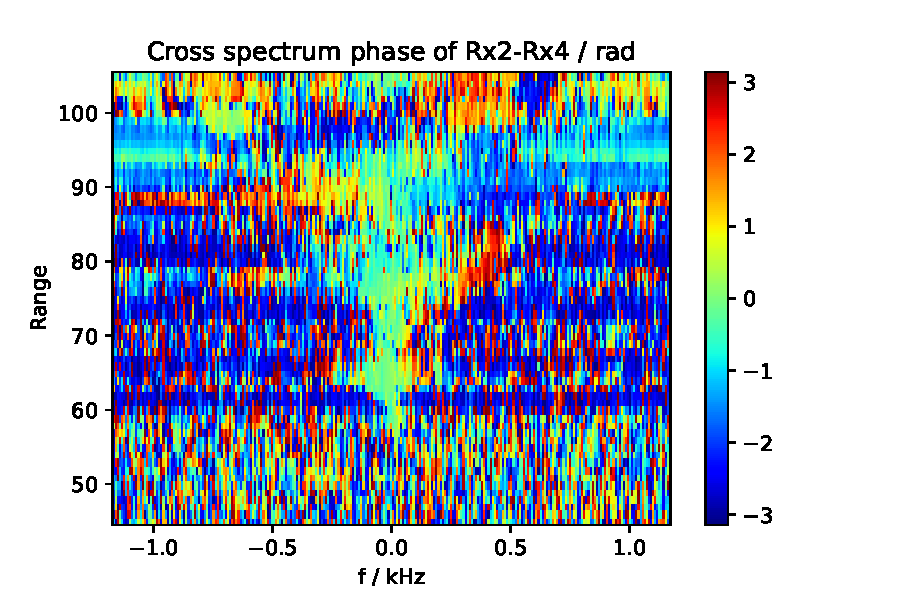
\includegraphics[width=\textwidth]{graphics/t4/t4-phase-2-4.pdf}
    \caption{Task 4: Phase of cross spectrum of Receivers 2 and 4.}
    \label{fig:t4-phase-2-4}
    \end{minipage}\hfill
    \begin{minipage}{0.48\textwidth}
        \centering
        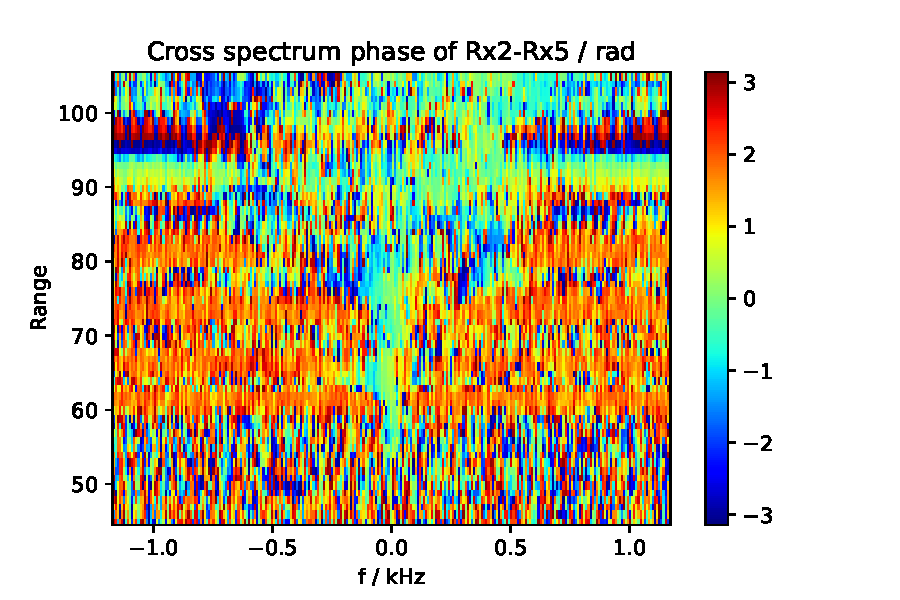
\includegraphics[width=\textwidth]{graphics/t4/t4-phase-2-5.pdf}
    \caption{Task 4: Phase of cross spectrum of Receivers 2 and 5.}
    \label{fig:t4-phase-2-5}
    \end{minipage}
\end{figure}

\begin{figure}[H]
    \centering
    \begin{minipage}{0.48\textwidth}
        \centering
        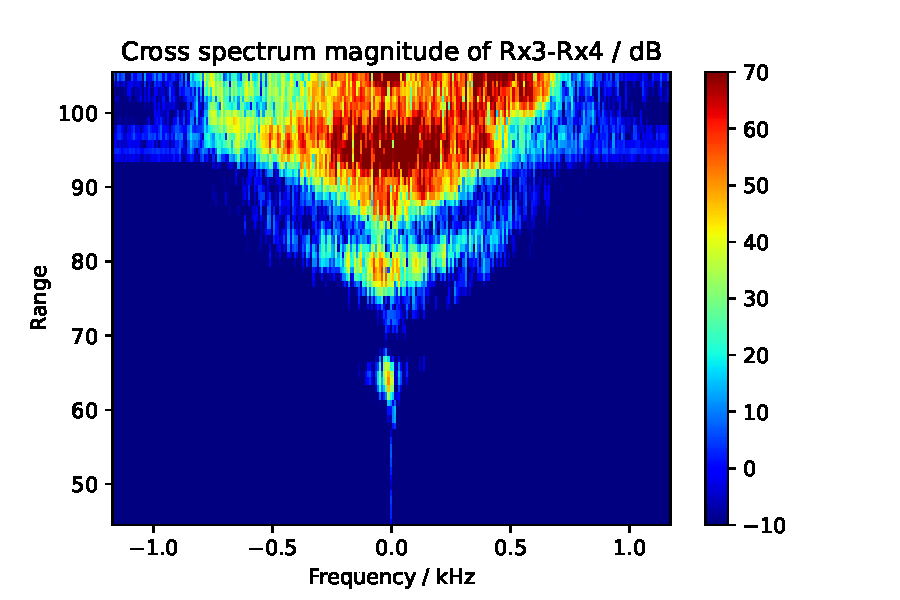
\includegraphics[width=\textwidth]{graphics/t4/t4-mag-3-4.pdf}
    \caption{Task 4: Magnitude of cross spectrum of Receivers 3 and 4.}
    \label{fig:t4-mag-3-4}
    \end{minipage}\hfill
    \begin{minipage}{0.48\textwidth}
        \centering
             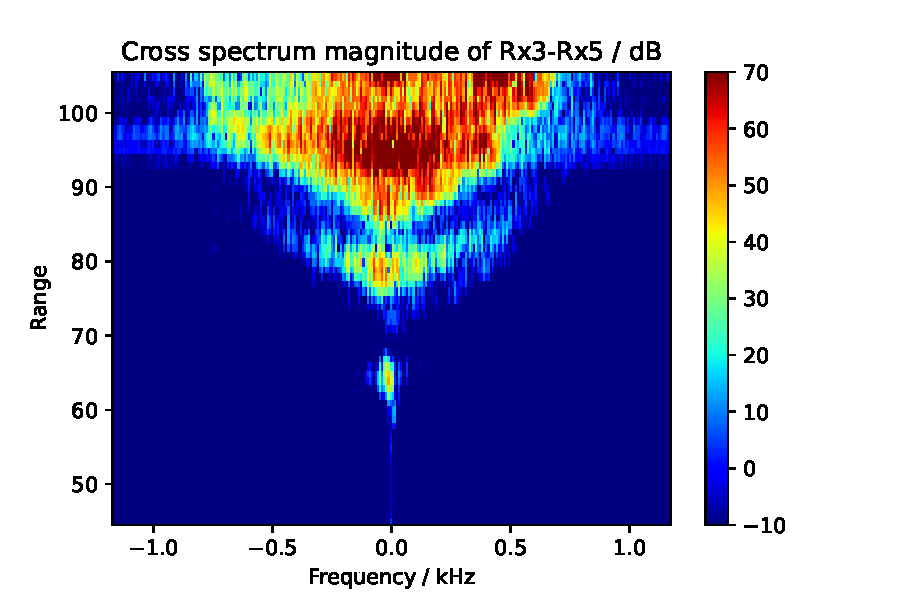
\includegraphics[width=\textwidth]{graphics/t4/t4-mag-3-5.pdf}
    \caption{Task 4: Magnitude of cross spectrum of Receivers 3 and 5.}
    \label{fig:t4-mag-3-5}
    \end{minipage}
\end{figure}

\begin{figure}[H]
    \centering
    \begin{minipage}{0.48\textwidth}
        \centering
        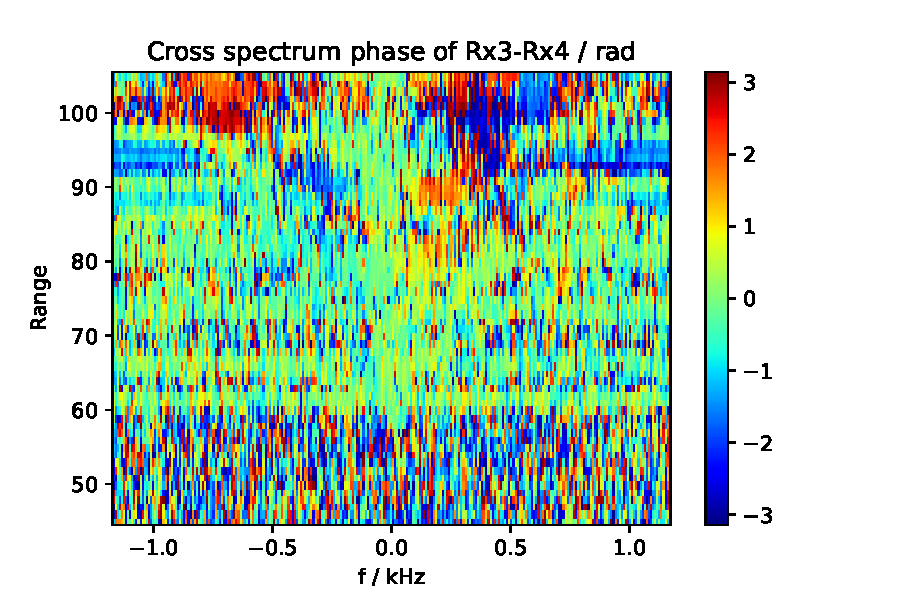
\includegraphics[width=\textwidth]{graphics/t4/t4-phase-3-4.pdf}
    \caption{Task 4: Phase of cross spectrum of Receivers 3 and 4.}
    \label{fig:t4-phase-3-4}
    \end{minipage}\hfill
    \begin{minipage}{0.48\textwidth}
        \centering
        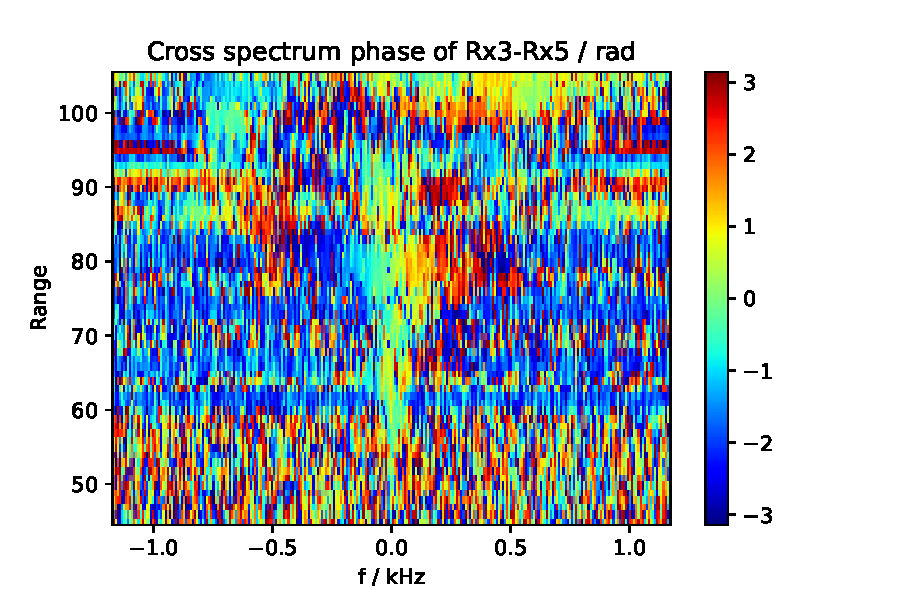
\includegraphics[width=\textwidth]{graphics/t4/t4-phase-3-5.pdf}
    \caption{Task 4: Phase of cross spectrum of Receivers 3 and 5.}
    \label{fig:t4-phase-3-5}
    \end{minipage}
\end{figure}


\end{document}
